\documentclass{article}
\PassOptionsToPackage{numbers,sort&compress}{natbib}
\usepackage[preprint]{neurips_2026}
\usepackage[utf8]{inputenc}
\usepackage[T1]{fontenc}
\usepackage{amsmath,amssymb,booktabs,graphicx,hyperref,url,microtype}
\hypersetup{hidelinks}
\newcommand{\RawN}{128,069}
\newcommand{\CleanN}{125,751}
\newcommand{\RemovedN}{2,318}
\newcommand{\FitN}{80,427}
\newcommand{\ValN}{19,969}
\newcommand{\TestN}{25,355}
\newcommand{\TrainN}{100,396}
\newcommand{\ChronoTrainN}{101,359}
\newcommand{\ChronoTestN}{24,392}
\newcommand{\BNFitSeconds}{0.446}
\newcommand{\QueryMinMS}{6.2}
\newcommand{\QueryMaxMS}{7.6}
\newcommand{\SearchMinSeconds}{0.21}
\newcommand{\SearchMaxSeconds}{0.24}
\newcommand{\EMK}{18}
\newcommand{\EMValLL}{0.65178}
\newcommand{\EMTestLL}{0.65854}
\newcommand{\EMHandAdvantage}{0.00245}
\newcommand{\EMHandLow}{0.00099}
\newcommand{\EMHandHigh}{0.00393}
\newcommand{\EMRestartN}{75}
\newcommand{\EMConvergedN}{66}
\newcommand{\EMCappedN}{9}
\newcommand{\EMFinalIter}{1000}
\newcommand{\PlayerN}{246}
\newcommand{\PlayerHalfN}{214}
\newcommand{\PlayerHalfR}{0.445}
\newcommand{\PlayerHalfDate}{2014-12-27}

\title{Expected Field Goal Probability:\\A Bayesian Network Model of NBA Shot Outcomes}
\author{Anna He \quad Fiona Feng \quad Hyeonung Cho \quad Logan Szeto\\
Group HALF \quad University of California, San Diego\\
CSE 150A/250A: Probabilistic Reasoning and Learning}
\begin{document}
\maketitle
\begin{center}\small\textbf{Working draft: individual contributions and reflections await team completion.}\end{center}

\begin{abstract}
We estimate NBA shot-make probabilities from observable shot circumstances using
Bayesian networks (BNs), with shooter and defender identities excluded. On
2014--15 shot logs, we compare a hand-designed BN, a BIC-learned BN, a latent-class
BN trained with EM, logistic regression, Naive Bayes, and a league-average baseline. The hand BN obtains
validation log loss 0.6505 and random-game test log loss 0.6561, versus 0.6594 for
logistic regression. We implement exact variable elimination and distinguish
graph-implied conditional-independence restrictions from empirical associations.
Conditional mutual information and paired game-cluster loss-difference intervals show
that Naive Bayes misses strong feature dependencies; adding every available
outcome parent can also hurt through sparse CPTs. Chronological robustness,
calibration, and supported probability queries illustrate both useful predictions
and limits of this observational shot-quality model. Player-level residuals are
exploratory comparisons against model expectations, rather than pure shooting skill.
\end{abstract}

\section{Problem Description}
Raw field goal percentage mixes the difficulty of attempted shots with the
shooter's ability. We define \emph{shot quality} as the estimated probability that
an observed shot is made given its circumstances: distance, point value, defender
proximity, shot-clock time, dribbles, and touch time. Our question is:
\textbf{How accurately can a BN predict outcomes, and which of its independence
assumptions provide useful approximations to observed shots?}

BNs make the dependency structure explicit and allow inference when some features
are unobserved \citep{koller}. Our contributions are a hand graph, smoothed CPT
estimation, custom exact inference, score-based structure learning, common-cohort
model comparisons, and analyses of independence, calibration, sparsity, and
robustness. Excluding player identity prevents direct use of individual shooting
percentages, but does not identify a universal league-average ability. Players
select their shots, so the estimand remains the make probability among the
observed attempts. Our claims are predictive and descriptive, not causal.

\section{Data Sourcing and Processing}
\subsection{Dataset and discretization}
The Kaggle NBA Shot Logs dataset \citep{dataset} contains \RawN{} attempts from
2014--15. The target $M$ is made/missed, mapped from \texttt{SHOT\_RESULT}.
We use six discrete predictors (Table~\ref{tab:variables}), excluding identities.
All intervals include their lower boundary and exclude their upper boundary.
Fixed bins are used across splits; no test values determine cutoffs.

\begin{table}[ht]
\centering\small
\caption{Model variables and states. Distances are feet; clock/touch time are seconds.}
\label{tab:variables}
\begin{tabular}{cll}
\toprule
Symbol & Description & States / interval boundaries\\
\midrule
$T$ & Recorded point value & $2,3$ (recorded, not derived from $D$)\\
$D$ & Shot distance & $[0,5),[5,10),\ldots,[25,30),[30,\infty)$\\
$C$ & Closest defender distance & $[0,2),[2,4),[4,6),[6,\infty)$\\
$S$ & Effective shot clock & $[0,4),[4,7),[7,15),[15,18),[18,22),[22,\infty)$\\
$B$ & Dribbles & $0,1,2,3$--$6,7+$\\
$H$ & Touch time & $[0,2),[2,6),[6,\infty)$\\
$M$ & Outcome & Missed $0$, made $1$\\
\bottomrule
\end{tabular}
\end{table}

\subsection{Data quality, splitting, and reproducibility}
There are 5,567 missing shot clocks and 3,857 recorded values of exactly 24.0.
For a missing clock with valid remaining period time in $[0,24]$, we retain the
shot and use that period time as a \emph{flagged proxy}; it is not a recovered
measurement. Missing clocks outside that window and invalid recorded clocks are
excluded. Valid observed clocks remain authoritative. Recorded 24.0 values are
retained and flagged as unverified; putback-like context does not prove the exact
release clock. Other invalid/missing target or feature values are removed.
Cleaning retains \CleanN{} shots, excluding \RemovedN{} overall.

We split by \texttt{GAME\_ID}, first reserving 20\% of games for test (seed 42),
then 20\% of the remaining games for validation (seed 123). Training-fit has
\FitN{} shots/578 games, validation \ValN{}/145, and test \TestN{}/181; outer
training combines training-fit and validation (\TrainN{}/723). These three
partitions have disjoint games and original-row IDs. The fixed chronological
check uses the earliest 80\% of unique dates for training and the remaining 20\%
for evaluation. This reuses the same cleaned dataset and is not external validation.
Earlier repository scripts already inspected the random-game test set; we do not
claim a pristine holdout. Subsequent model choices use training/validation.

Raw-row IDs are assigned before cleaning and scoped to the raw-file SHA256.
Preprocessing and experiment metadata record input/output/source hashes, package
versions, code revision, bins, clock policy, seeds, and counts. Shared loaders
reject stale inputs, overlapping cohorts, and mismatched learned-graph files.
This resolved a saved-calibration mismatch of 20,175 versus 19,969 validation shots.

\section{Modeling and Inference}
\subsection{Hand graph and parameter learning}
Figure~\ref{fig:graphs} compares the hand graph and the graph learned on
training-fit data. The hand joint distribution is
\begin{align}
P(S,D,B,H,T,C,M)={}&P(S)P(D)P(B\mid S)P(H\mid S,B)\nonumber\\
&\cdot P(T\mid D)P(C\mid D,B)P(M\mid D,T,C,H).
\end{align}
Thus it assumes $M\perp(S,B)\mid D,T,C,H$ and marginal independence of roots
$S$ and $D$. These are imposed model restrictions, not established data facts.
Graph definitions are shared by all hand-model implementations.

\begin{figure}[ht]
\centering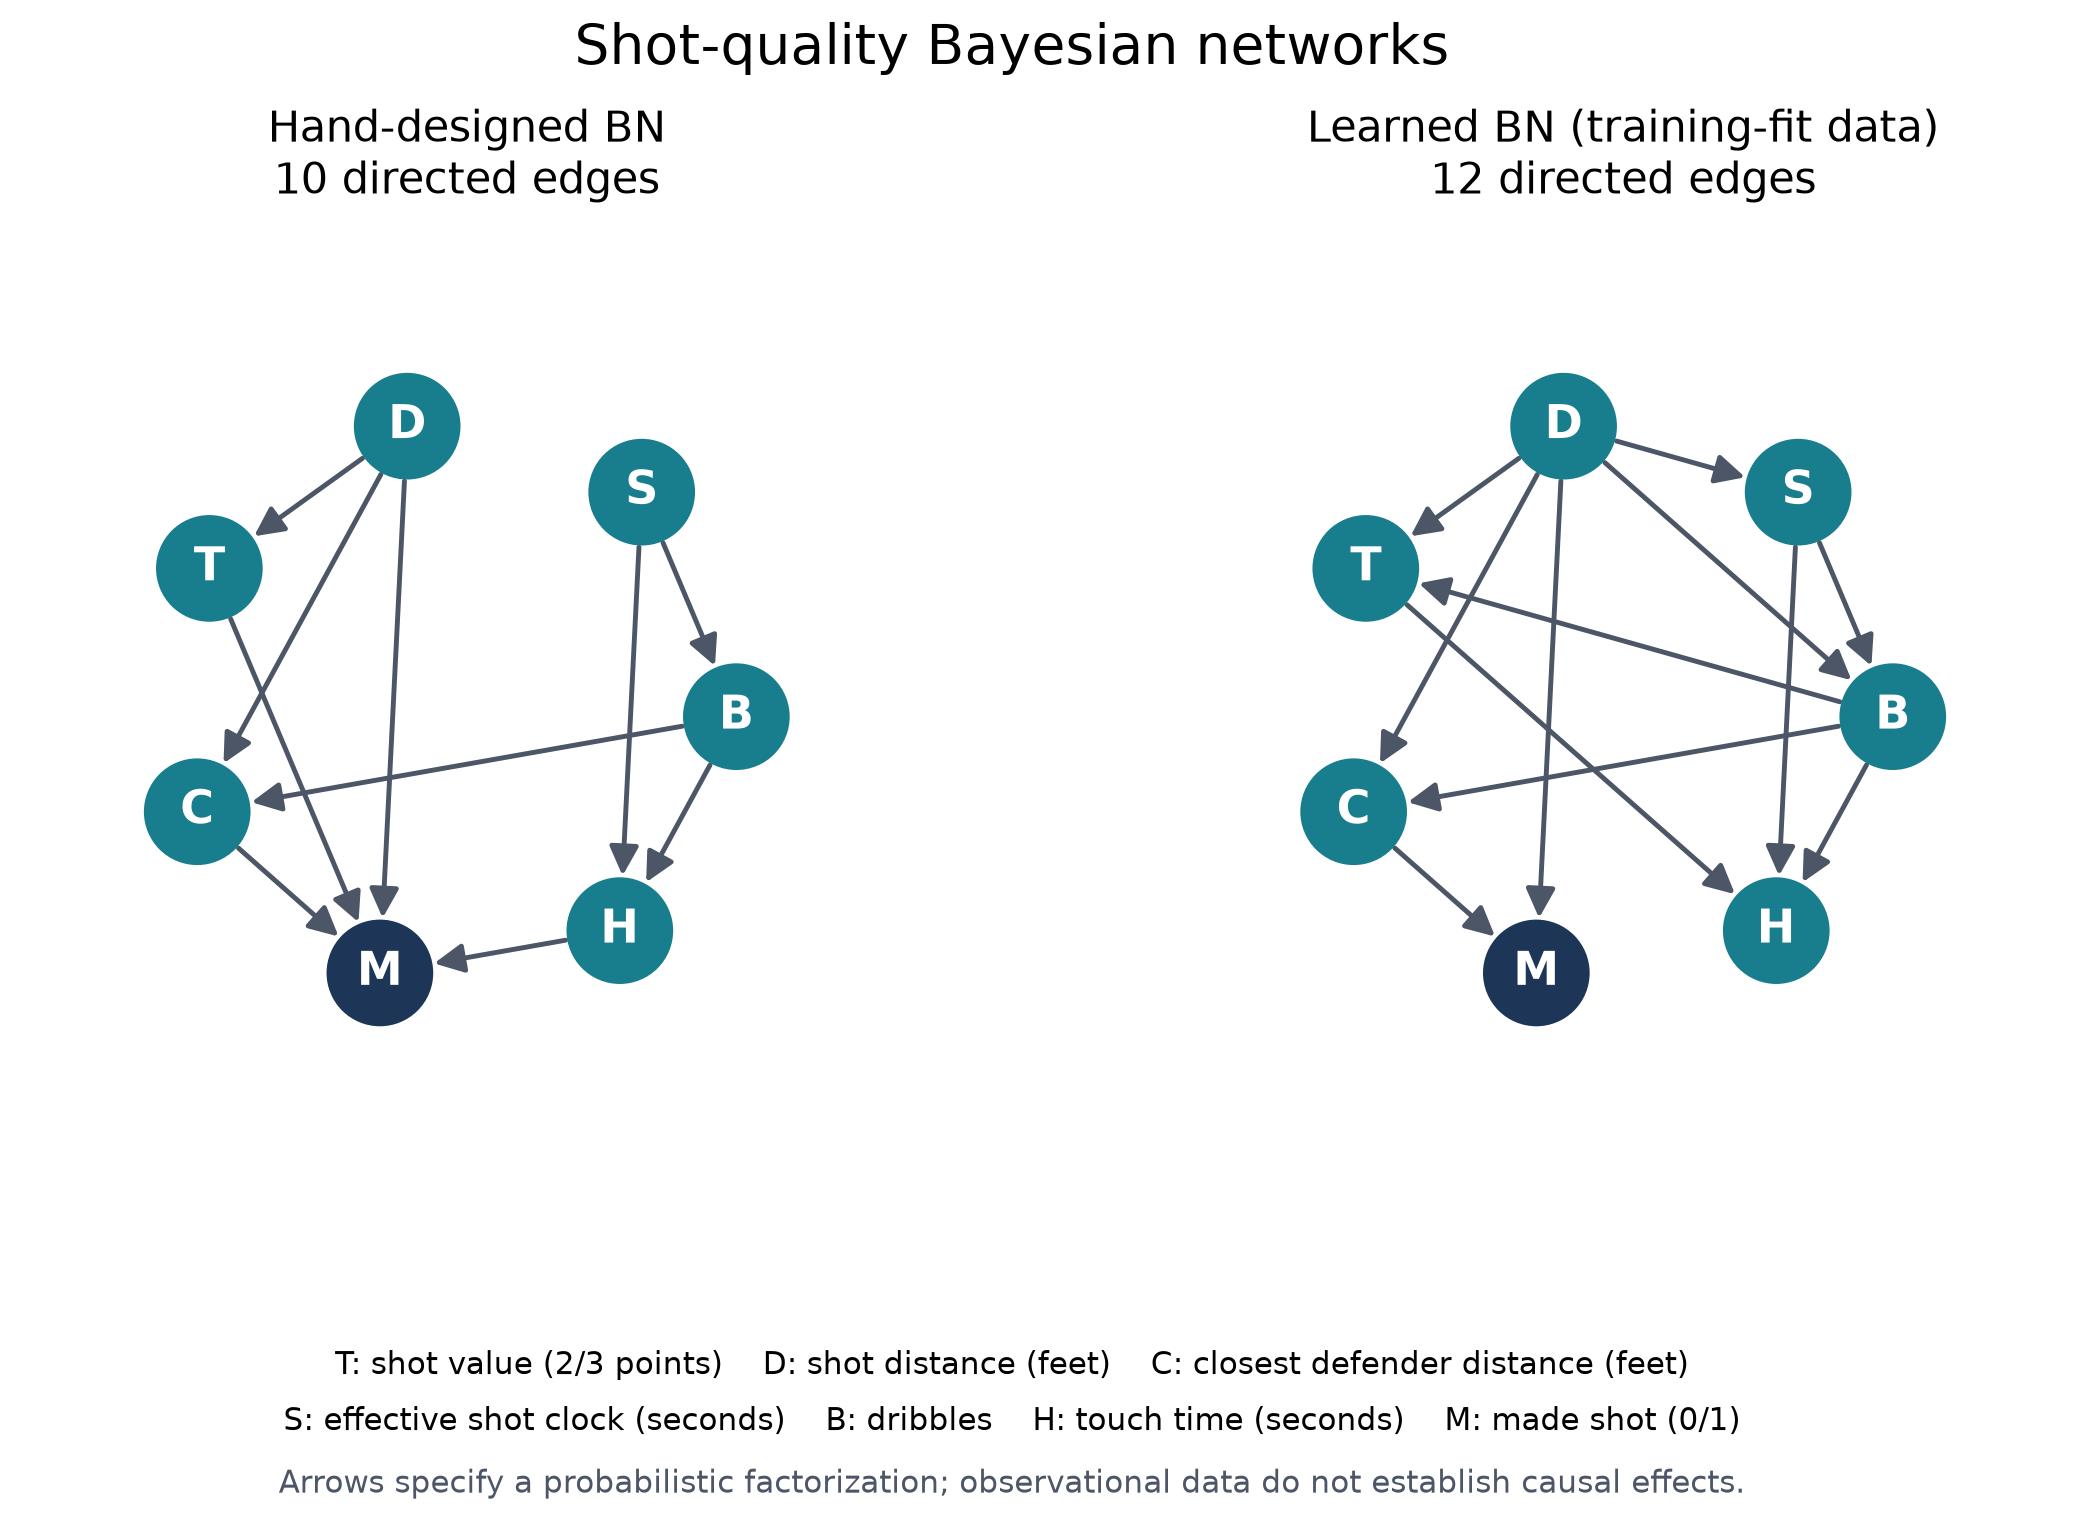
\includegraphics[width=0.82\linewidth]{../results/figures/bayesian_network_graphs.png}
\caption{Actual hand and training-fit learned DAGs. Symbols are defined in
Table~\ref{tab:variables}. Directions specify a factorization and are not identified causal effects.}
\label{fig:graphs}
\end{figure}

Each CPT uses a symmetric Dirichlet prior with $\alpha=1$. For node state $x$
and parent configuration $\pi$, the posterior mean is
$\hat P(x\mid\pi)=(N_{x,\pi}+\alpha)/(N_\pi+r_x\alpha)$.
In particular, $\hat P(M=1\mid d,t,c,h)=(N_1+1)/(N+2)$.
This is Laplace smoothing, not unsmoothed MLE. An unobserved binary parent
configuration receives probability $1/2$. More parents increase both flexibility
and the product of parent-state cardinalities, potentially producing unreliable
rows. For observed make-CPT rows we also report Beta$(N_1+1,N_0+1)$ equal-tailed
95\% intervals; these use an independent-shot likelihood and are not cluster-adjusted.

\subsection{Exact inference, structure learning, and baselines}
Our variable-elimination implementation restricts factors to evidence, multiplies
relevant factors, sums out hidden variables, and normalizes. It answers partial
queries such as $P(M=1\mid D,C,T)$ by marginalizing unobserved $S,B,H$.
Synthetic tests check it against full-joint enumeration and verify make-CPT
identities when all make parents are observed. Under fully observed predictors,
$M$ is a leaf and only its parent CPT is needed for outcome prediction; the
remaining graph matters for partial evidence and joint interpretation.

We use pgmpy hill climbing \citep{pgmpy} with discrete BIC \citep{schwarz}, at most
four parents per node, and no outgoing edges from $M$. The training-fit learned
make parents are $C,D$; BIC scores the full joint factorization with a complexity
penalty, rather than directly minimizing held-out outcome log loss. Greedy search
can find a local solution. A fixed Python hash seed makes tie ordering repeatable.

Baselines are the training make rate, one-hot logistic regression (unknown states
ignored, 1,000 maximum optimizer iterations), and custom discrete Naive Bayes
with Laplace smoothing. Naive Bayes factorizes
$P(M)\prod_jP(X_j\mid M)$, imposing feature independence conditional on outcome.
We use scikit-learn for logistic regression and metrics \citep{sklearn} and the
scientific Python stack for tables, graphs, and figures \citep{software}.

The latent-class extension introduces $Q$ as a parent of all six
features and $M$. MAP-EM fits $K=2,\ldots,10,12,14,16,18,20$, with five seeded
restarts per $K$. We retain each $K$'s highest training posterior objective, then
select $K$ by validation log loss and refit on outer training. Prediction
marginalizes $Q$ using features alone. Add-one pseudocounts here correspond to
a Dirichlet$(2)$ MAP update. Appendix~\ref{sec:extensions} records convergence,
latent-state interpretation, and the separate five-fold game-cross-fitted
player analysis.

\subsection{Independence diagnostics and uncertainty}
We first verify graph restrictions by d-separation. We then measure plug-in
conditional mutual information (CMI, natural-log units) on complete training-fit
cases:
\begin{equation}
\widehat I(X;Y\mid Z)=\sum_{x,y,z}\frac{n_{xyz}}N
\log\frac{n_{xyz}n_z}{n_{xz}n_{yz}}.
\end{equation}
Joint-variable claims are encoded jointly; pairwise independence does not imply
joint independence. We report within-stratum state counts, empty cells, small
expected counts, and constant strata. Finite-sample CMI is upward biased,
especially in sparse tables. The descriptive statistic $2N\widehat I$ is not
assigned an ordinary chi-square p-value: shots are clustered and table support
can be inadequate. Positive CMI alone is not a formal rejection of independence.

Matched parent-set models are fitted on training-fit and evaluated on identical
validation shots. For predictive relevance we use paired game-cluster bootstrap
intervals: sample 145 games with replacement, retain all their shots (including
multiplicity), and average paired shot-loss differences. We use 1,000 draws,
seed 20261117, and percentile 2.5/97.5 limits, accommodating within-game
association \citep{cluster}. Intervals condition on fitted models and earlier
validation selection; they omit refitting uncertainty and cross-game player
dependence. Final primary-versus-baseline comparisons use the same procedure on
181 test games. These are nominal pairwise intervals without multiplicity adjustment.
No final-test or chronological-evaluation outcome chooses a model or tuning parameter.

\section{Results and Discussion}
\subsection{Common-cohort prediction and calibration}
Table~\ref{tab:main} uses the synchronized validation set, then refits each fixed
model on all outer-training shots for the common random-game test. Accuracy uses
a 0.5 threshold; Brier score is the mean squared probability error. ECE is the
count-weighted absolute gap between predicted and observed make rates in ten
equal-width bins. We prioritize log loss and Brier score; ECE alone does not
measure discrimination, and its value depends on binning.

\begin{table}[ht]
\caption{Synchronized validation and final random-game test results. LL denotes
log loss. Lower LL/Brier/ECE and higher accuracy are better.}
\label{tab:main}\centering\small\begin{tabular}{lrrrrr}
\toprule
Model & Val. LL & Test LL & Test Brier & Test Acc. & Test ECE\\
\midrule
Hand BN & 0.6505 & 0.6561 & 0.2322 & 0.6142 & 0.0055\\
Latent BN ($K=18$) & 0.6518 & 0.6585 & 0.2334 & 0.6058 & 0.0074\\
Learned BN & 0.6527 & 0.6593 & 0.2337 & 0.6086 & 0.0062\\
Logistic regression & 0.6528 & 0.6594 & 0.2336 & 0.6093 & 0.0260\\
Naive Bayes & 0.6671 & 0.6752 & 0.2402 & 0.6039 & 0.0523\\
League average & 0.6880 & 0.6896 & 0.2482 & 0.5426 & 0.0060\\
\bottomrule
\end{tabular}

\end{table}

The hand BN has the lowest observed test log loss. Its paired test advantage over
logistic regression is 0.00336 (95\% game-cluster interval [0.00202,0.00465]) and
over the learned BN is 0.00324 ([0.00229,0.00422]); these are modest conditional
comparisons, not evidence of universal superiority. The learned graph's richer
feature structure does not guarantee better fully observed outcome prediction.
The league baseline has low ECE but assigns every shot the same probability;
its worse proper scoring rules expose that limitation. Naive Bayes has noticeably
poorer calibration (test ECE 0.0523). Reliability curves and bin-support counts
are supplied in the appendix and saved figures; sparse extreme bins should not
be overinterpreted.

\subsection{Independence assumptions versus observed dependence}
Table~\ref{tab:ci} measures the predeclared restrictions on \FitN{} training-fit
shots; no selected variable is missing in this cleaned cohort. All restrictions
are verified in their respective graphs, but data associations remain.

\begin{table}[ht]
\caption{Descriptive CMI and percentage of all analyzed shots lying in informative
strata with any expected cell count below five. CMI is not a formal cluster-valid CI test.}
\label{tab:ci}\centering\small\begin{tabular}{lrr}
\toprule
Graph restriction & CMI (nats) & Sparse shots\\
\midrule
$M\perp S\mid D,T,C,H$ & 0.00495 & 29.9\%\\
$M\perp B\mid D,T,C,H$ & 0.00260 & 71.3\%\\
$M\perp(S,B)\mid D,T,C,H$ & 0.01482 & 99.9\%\\
$S\perp D$ & 0.05685 & 0.0\%\\
$D\perp T\mid M$ & 0.40880 & 0.0\%\\
$B\perp H\mid M$ & 0.55395 & 0.0\%\\
$M\perp H\mid D,C$ & 0.00255 & 1.7\%\\
$M\perp(T,S,B,H)\mid D,C$ & 0.01812 & 100.0\%\\
\bottomrule
\end{tabular}

\end{table}

The Naive Bayes restrictions have large CMI for distance/point value (0.4088) and
dribbles/touch time (0.5539), with well-supported tables within each outcome stratum. Redundant
feature evidence is a plausible explanation for its overconfident probabilities.
The hand graph's independent roots also miss shot-clock/distance association
(CMI 0.0569), an issue relevant to partial-evidence inference even when the fully
observed make CPT performs well. The high-dimensional joint claims place almost
all shots in sparse strata; their positive plug-in CMI is therefore interpreted
alongside predictive sensitivity, not as a reliable population-independence test.

\subsection{Ablations, predictive sensitivity, and sparsity}
Removing distance increases validation log loss from 0.65051 to 0.67351; removing
defender distance gives 0.65899 and removing touch time gives 0.65248. These
matched ablations identify useful predictors without proving conditional dependence.
Adding shot clock improves validation log loss by only 0.00020, with an interval
spanning zero. Adding dribbles alone also has an interval spanning zero. Adding
both worsens loss by 0.00424 (95\% interval for improvement
[$-0.00606$,$-0.00260$]); the six-parent CPT has 5,040 possible configurations but
only 1,839 observed, and 0.48\% of validation shots fall in unseen configurations.
Adding touch time to learned parents $C,D$ improves validation loss by 0.00201
([0.00088,0.00315]). This challenges its omitted-touch-time restriction in a
predictive sense, while the comparison remains exploratory after validation use.
We retain the original hand graph as the primary fixed, interpretable model;
the clock-augmented alternative is a sensitivity result.

\begin{figure}[ht]
\centering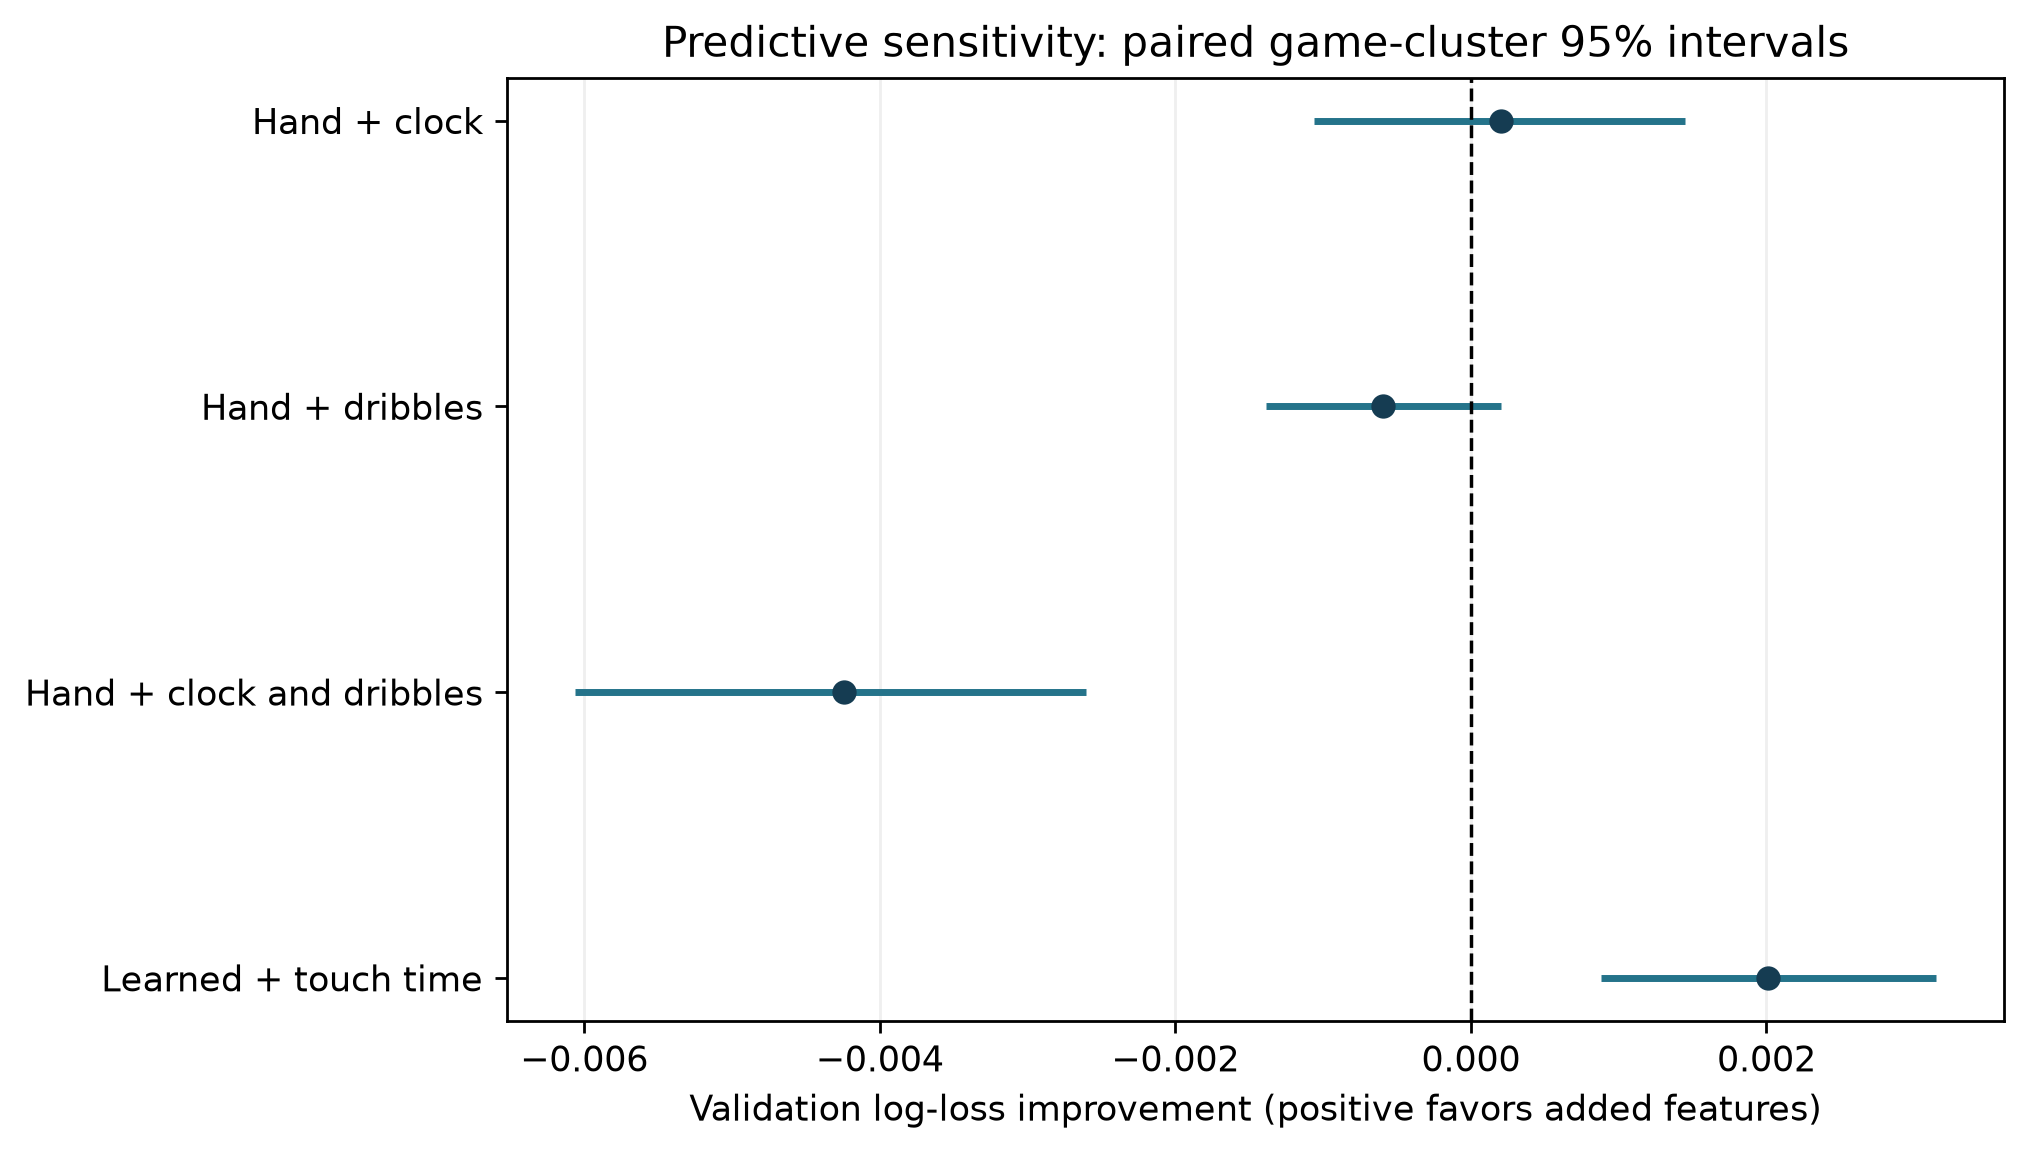
\includegraphics[width=0.90\linewidth]{../results/figures/ci_predictive_sensitivity.png}
\caption{Paired game-cluster intervals on the validation cohort. Positive values
favor expanded parent sets. These intervals are conditional on already fitted models.}
\label{fig:sensitivity}
\end{figure}

\subsection{Latent-class and player extensions}
Validation selects $K=\EMK{}$ latent states (log loss \EMValLL{}); refitting on
the same outer training gives test log loss \EMTestLL{}. The hand model's
paired advantage is \EMHandAdvantage{} (95\% game-cluster interval
[\EMHandLow{},\EMHandHigh{}]). The latent model captures dependence through
$Q$ but does not improve this test comparison. This is an exploratory
validation-selected extension. The selected outer-training fit reaches the
1,000-evaluation cap without meeting tolerance, limiting this comparison.

Five-fold game cross-fitting gives descriptive actual-minus-expected player
residuals. Among \PlayerHalfN{} players with at least 100 attempts in each half,
independently fitted within-half residuals correlate at $r=\PlayerHalfR{}$.
This analysis uses all cleaned games, including the earlier test cohort; it is
separate from held-out prediction assessment. Omitted context and model error
also contribute to residuals, so persistence does not isolate shooting skill.
Full procedures, support counts, and illustrative players are in
Appendix~\ref{sec:extensions}.

\subsection{Chronological robustness and preprocessing sensitivity}
Training on October 28, 2014--February 2, 2015 (\ChronoTrainN{} shots/720 games)
and evaluating February 3--March 4, 2015 (\ChronoTestN{}/184) yields
Table~\ref{tab:chrono}. The learned graph is relearned only on the earlier training dates. The
hand model has the lowest observed log loss among the five evaluated models.
This check covers the five observed-variable models; latent EM is evaluated on
the random-game cohort only. Both
this run and the fixed training-fit run select make parents $C,D$ for the learned
BN; earlier saved results had differed under older experiments.

\begin{table}[ht]
\caption{Reproduced chronological robustness results; the cohort reuses the
original cleaned data and is not independent external validation.}
\label{tab:chrono}\centering\small\begin{tabular}{lrrrr}
\toprule
Model & Log loss & Brier & Accuracy & ECE\\
\midrule
Hand BN & 0.6525 & 0.2306 & 0.6204 & 0.0091\\
Learned BN & 0.6549 & 0.2317 & 0.6147 & 0.0087\\
Logistic regression & 0.6547 & 0.2314 & 0.6122 & 0.0208\\
Naive Bayes & 0.6715 & 0.2385 & 0.6059 & 0.0540\\
League average & 0.6875 & 0.2472 & 0.5536 & 0.0077\\
\bottomrule
\end{tabular}

\end{table}

Training-only diagnostics also compare fixed and training-fitted quantile distance
bins, plus treatments of recorded 24.0 shot clocks. The five game-level validation
splits overlap, so their means are sensitivity summaries rather than independent
replications. The current 30+ distance scheme has the lowest mean log loss for all
three models: hand BN 0.65215 versus 0.65416 with the original bins and 0.65286
with training-fitted quantiles (Table~\ref{tab:preprocessing}). Separating 24.0
changes logistic log loss by only $-0.000007$ and Naive Bayes by $+0.000218$.
Changing shot-clock categories leaves the hand make CPT unchanged
because $S$ is not its parent. A missing-category treatment and a separately named
24.0 category convey the same categorical distinction to these baseline models;
neither verifies the underlying release clock.

\subsection{Inference, stability, and scalability}
Supported partial-evidence queries are in Table~\ref{tab:queries}. The near-basket
wide-open query gives 0.935 versus 0.515 for tight defense, with 899 and 8,273
supporting shots respectively. These are associational mixtures, potentially
including dunks and different shooter populations, not effects of moving a defender.
The full hand BN fits in \BNFitSeconds{} seconds and the four fixed queries take
\QueryMinMS{}--\QueryMaxMS{} milliseconds each on this machine (single runs).
Three fixed 80\% subsamples of training-fit games all retain make parents $C,D$,
with 11--12 total edges and search times \SearchMinSeconds{}--\SearchMaxSeconds{}
seconds. Other directed edges vary; three overlapping subsamples are not
confidence levels for a true graph. Greedy stopping does not certify a global optimum.

CPT estimation is finite counting, not iterative convergence. Exact inference
cost depends on elimination order and intermediate-factor cardinalities. Adding
parents expands CPTs multiplicatively, so more data can stabilize rare observed
strata but cannot repair missing features or causal identification. Other limits
include coarse bins, unmeasured shot type/location/context, only attempted shots,
player dependence across games, and coverage of only part of one season.

\clearpage
\section{Conclusion}
A small, interpretable hand BN gives useful outcome probabilities and competitive
calibration on common cohorts, while exact inference supports incomplete evidence.
The project connects factorization, smoothed CPT learning, d-separation, exact
marginalization, and score-based search to observed data. Independence analysis
shows why model restrictions must be checked rather than read as facts: strong
feature dependence plausibly contributes to Naive Bayes miscalibration, weak outcome additions may not improve
prediction, and unrestricted parent expansion creates sparsity. Richer defensive
features, additional seasons, and hierarchical player effects are useful future
directions. Latent classes and player residuals broaden the analysis but do not
resolve unobserved context or identify player skill.

\section{Reflections and Contributions}
\textbf{Team completion required.} Each member must supply a truthful 1--2 sentence
account of their own tasks and a brief individual reflection; none is inferred
from author order or fabricated from code history.
\paragraph{Anna He.} \textit{Awaiting Anna's contribution statement and personal reflection.}
\paragraph{Fiona Feng.} \textit{Awaiting Fiona's contribution statement and personal reflection.}
\paragraph{Hyeonung Cho.} \textit{Awaiting Hyeonung's contribution statement and personal reflection.}
\paragraph{Logan Szeto.} \textit{Awaiting Logan's contribution statement and personal reflection.}
\paragraph{Advice and iteration.} Preserve original-row identity, keep game-level
partitions separate, compare proper probability scores on identical shots, and
inspect sparse CPT rows before adding features. A useful iteration here was
reconciling stale calibration artifacts before drawing model comparisons.
\paragraph{AI assistance disclosure.} Codex assisted with repository review,
preprocessing provenance, graph/CMI diagnostics, game-cluster uncertainty,
common-cohort evaluation, EM/player integration, tests, figures, and revisions to this supplied LaTeX
draft. Team members must review, adapt, and be able to explain the final code,
analysis, and prose under the course policy before submission.

\clearpage
\begin{thebibliography}{9}
\raggedright
\bibitem{dataset} D. Becker. \emph{NBA Shot Logs (2014--15 season)}. Kaggle.
\url{https://www.kaggle.com/datasets/dansbecker/nba-shot-logs}.
\bibitem{koller} D. Koller and N. Friedman. \emph{Probabilistic Graphical Models:
Principles and Techniques}. MIT Press, 2009.
\url{https://mitpress.mit.edu/9780262013192/probabilistic-graphical-models/}.
\bibitem{schwarz} G. Schwarz. Estimating the dimension of a model.
\emph{Annals of Statistics}, 6(2):461--464, 1978.
\url{https://doi.org/10.1214/aos/1176344136}.
\bibitem{cluster} A. C. Cameron and D. L. Miller. A practitioner's guide to
cluster-robust inference. \emph{Journal of Human Resources}, 50(2):317--372, 2015.
\url{https://doi.org/10.3368/jhr.50.2.317}.
\bibitem{pgmpy} pgmpy developers. \emph{pgmpy documentation and source}.
Version 1.1.2 used for structure learning.
\url{https://pgmpy.org/}; \url{https://github.com/pgmpy/pgmpy}.
\bibitem{sklearn} F. Pedregosa et al. Scikit-learn: Machine learning in Python.
\emph{Journal of Machine Learning Research}, 12:2825--2830, 2011.
\url{https://www.jmlr.org/papers/v12/pedregosa11a.html}.
\bibitem{software} Scientific Python tools: NumPy, \url{https://numpy.org/};
pandas, \url{https://pandas.pydata.org/}; SciPy, \url{https://scipy.org/};
Matplotlib, \url{https://matplotlib.org/}; NetworkX, \url{https://networkx.org/}.
Exact installed versions and source checksums accompany each experiment.
\end{thebibliography}

\clearpage\appendix
\raggedbottom
\section{Supported inference and uncertainty summaries}
\begin{table}[!ht]
\caption{Partial-evidence queries from the full hand BN trained on training-fit
shots; touch time, shot clock, and dribbles are marginalized where unobserved.}
\label{tab:queries}\centering\small\begin{tabular}{lrrr}
\toprule
Evidence & Shots & Observed & BN query\\
\midrule
No evidence & 80,427 & 0.452 & 0.453\\
$D<5,T=2,C<2$ & 8,273 & 0.516 & 0.515\\
$D<5,T=2,C\geq6$ & 899 & 0.940 & 0.935\\
$25\leq D<30,T=3,4\leq C<6$ & 2,973 & 0.323 & 0.323\\
\bottomrule
\end{tabular}

\end{table}
\begin{table}[!ht]
\caption{Validation sensitivity. Positive difference favors the expanded parent set.}
\centering\small\begin{tabular}{lrr}
\toprule
Added parents & $\Delta$ log loss & 95\% game interval\\
\midrule
Hand: clock & +0.00020 & [-0.00106, +0.00145]\\
Hand: dribbles & -0.00059 & [-0.00139, +0.00021]\\
Hand: clock and dribbles & -0.00424 & [-0.00606, -0.00260]\\
Learned: touch time & +0.00201 & [+0.00088, +0.00315]\\
\bottomrule
\end{tabular}

\end{table}
\begin{table}[!ht]
\caption{Random-game test paired loss differences. Positive values favor the hand
BN over the comparator. Limits are conditional game-cluster percentile intervals.}
\centering\small\begin{tabular}{lrr}
\toprule
Comparator & Hand advantage & 95\% game interval\\
\midrule
League average & +0.03351 & [+0.03016, +0.03691]\\
Logistic regression & +0.00336 & [+0.00202, +0.00465]\\
Naive Bayes & +0.01910 & [+0.01668, +0.02143]\\
Learned BN & +0.00324 & [+0.00229, +0.00422]\\
Latent BN & +0.00245 & [+0.00099, +0.00393]\\
\bottomrule
\end{tabular}

\end{table}
\begin{table}[!ht]
\caption{Mean validation log loss across five overlapping game-level splits of
outer training. These are descriptive sensitivity summaries, not independent replications.}
\label{tab:preprocessing}\centering\small\begin{tabular}{lrrr}
\toprule
Distance scheme & Hand BN & Logistic & Naive Bayes\\
\midrule
Original six bins & 0.65416 & 0.65590 & 0.67106\\
Five-foot, 25+ & 0.65268 & 0.65458 & 0.66990\\
Five-foot, 30+ (used) & 0.65215 & 0.65414 & 0.66939\\
Seven training quantiles & 0.65286 & 0.65491 & 0.67092\\
\bottomrule
\end{tabular}

\end{table}
\begin{figure}[ht]
\centering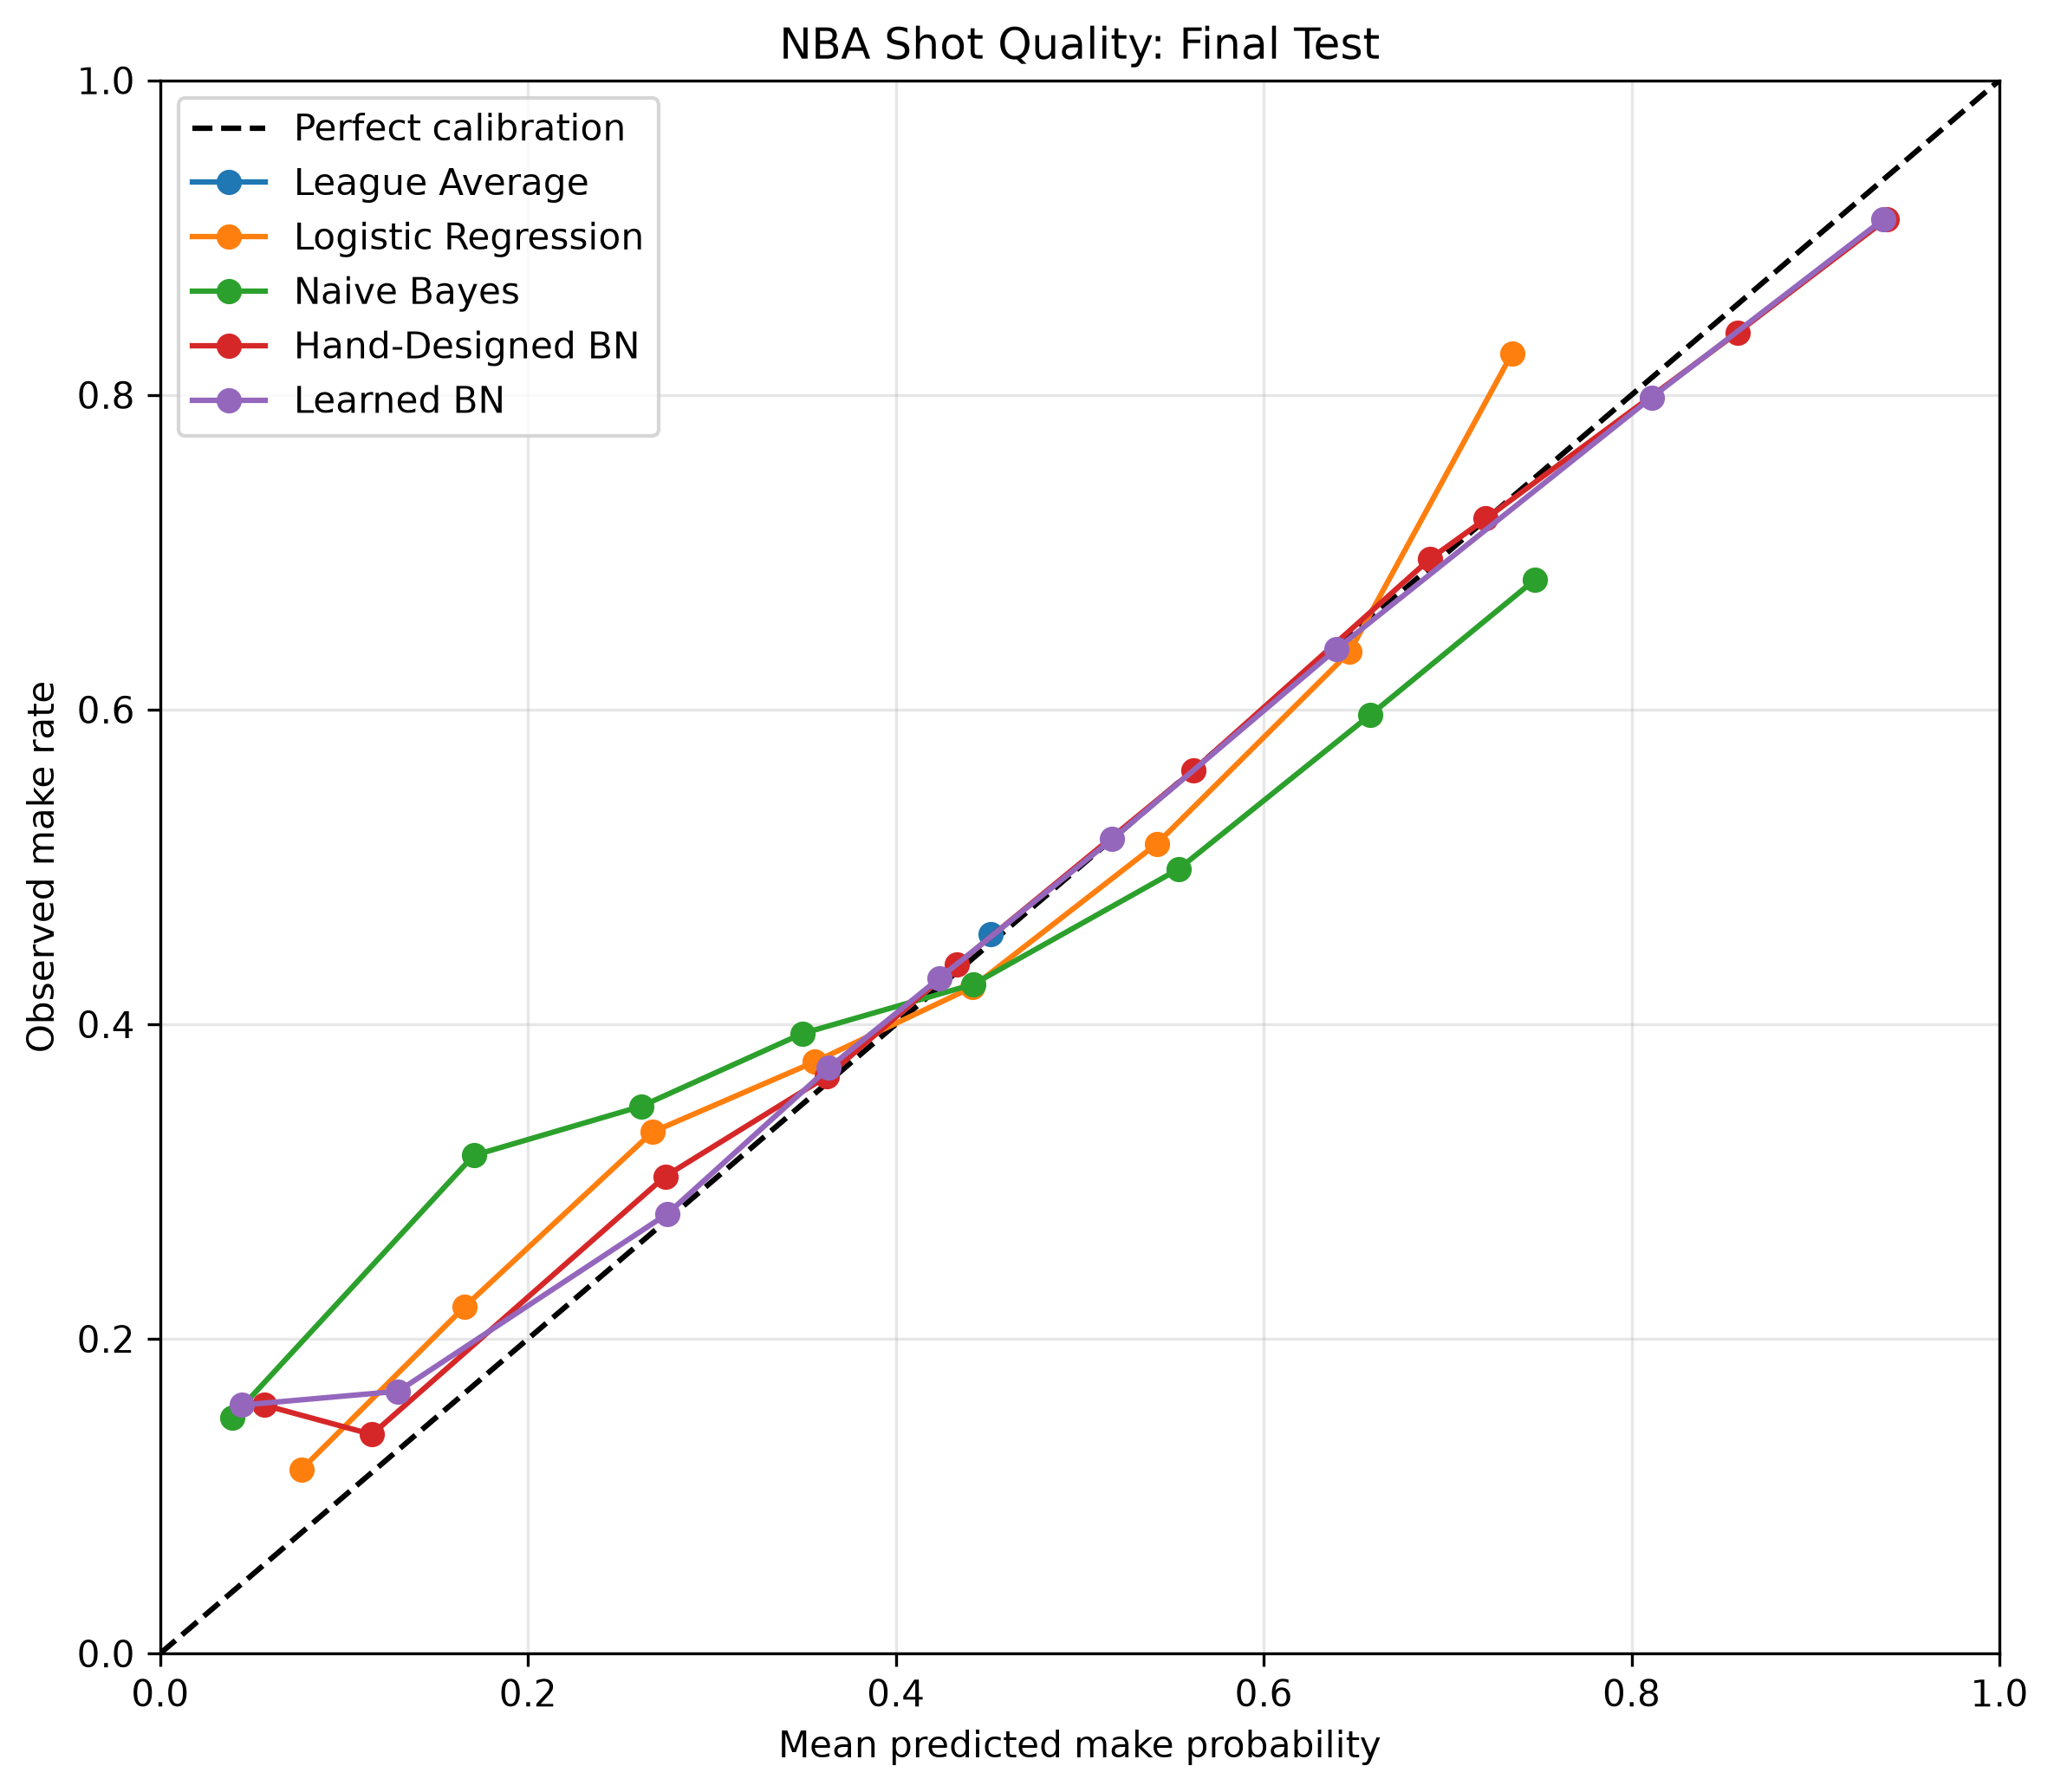
\includegraphics[width=0.8\linewidth]{../results/figures/final_test_calibration.png}
\caption{Final-test reliability curves for the five observed-node models. The corresponding bin counts are
saved in \texttt{final\_test\_calibration\_bins.csv}; rare bins have larger uncertainty.}
\end{figure}

\clearpage
\section{Latent-class and player extensions}\label{sec:extensions}
These extensions incorporate Anna's merged implementation with the same
hash-verified preprocessing and split identities used by the core experiments.

\subsection{Latent-variable modeling with MAP-EM}
A hidden categorical variable $Q$ represents statistical shot configurations:
\[P(Q,M,X_1,\ldots,X_6)=P(Q)P(M\mid Q)\prod_{i=1}^{6}P(X_i\mid Q).\]
The E-step computes $r_{iq}\propto P(q)P(m_i\mid q)\prod_jP(x_{ij}\mid q)$.
The M-step uses expected counts with add-one pseudocounts for every prior/CPT
state, maximizing a Dirichlet$(2)$ posterior objective. During prediction,
$P(q\mid x_i)$ excludes $m_i$ and $P(M=1\mid x_i)=\sum_qP(q\mid x_i)P(M=1\mid q)$.
An unseen feature value is marginalized rather than assigned an arbitrary code.

We preserve the 14-value $K$ grid and five restarts (seeds 0--4), selecting each
$K$'s restart by training posterior objective and then $K$ by validation log loss.
The selected $K=\EMK{}$ is refitted using five restarts on all outer training;
the test set never selects $K$ or a restart. BIC at the MAP fit is descriptive,
not the selection criterion; finite mixtures need not satisfy regular BIC assumptions.

Stopping requires objective improvement below $10^{-7}$ per training shot,
with a 1,000-evaluation cap. Material objective decreases raise an error. Of
\EMRestartN{} selection/refit runs, \EMConvergedN{} meet the tolerance and
\EMCappedN{} hit the cap. The selected final fit reaches \EMFinalIter{} evaluations
without meeting tolerance; its capped result is retained under the fixed protocol.
Recorded likelihoods/objectives correspond to the returned parameters, including
at the cap. Identical observed tuples are frequency-compressed after the original
per-shot initialization; weighted EM preserves the full shot likelihood and
updates. Detailed traces and identified predictions are reproducible local
artifacts; compact restart summaries and metadata accompany the committed results.

\begin{figure}[ht]
\centering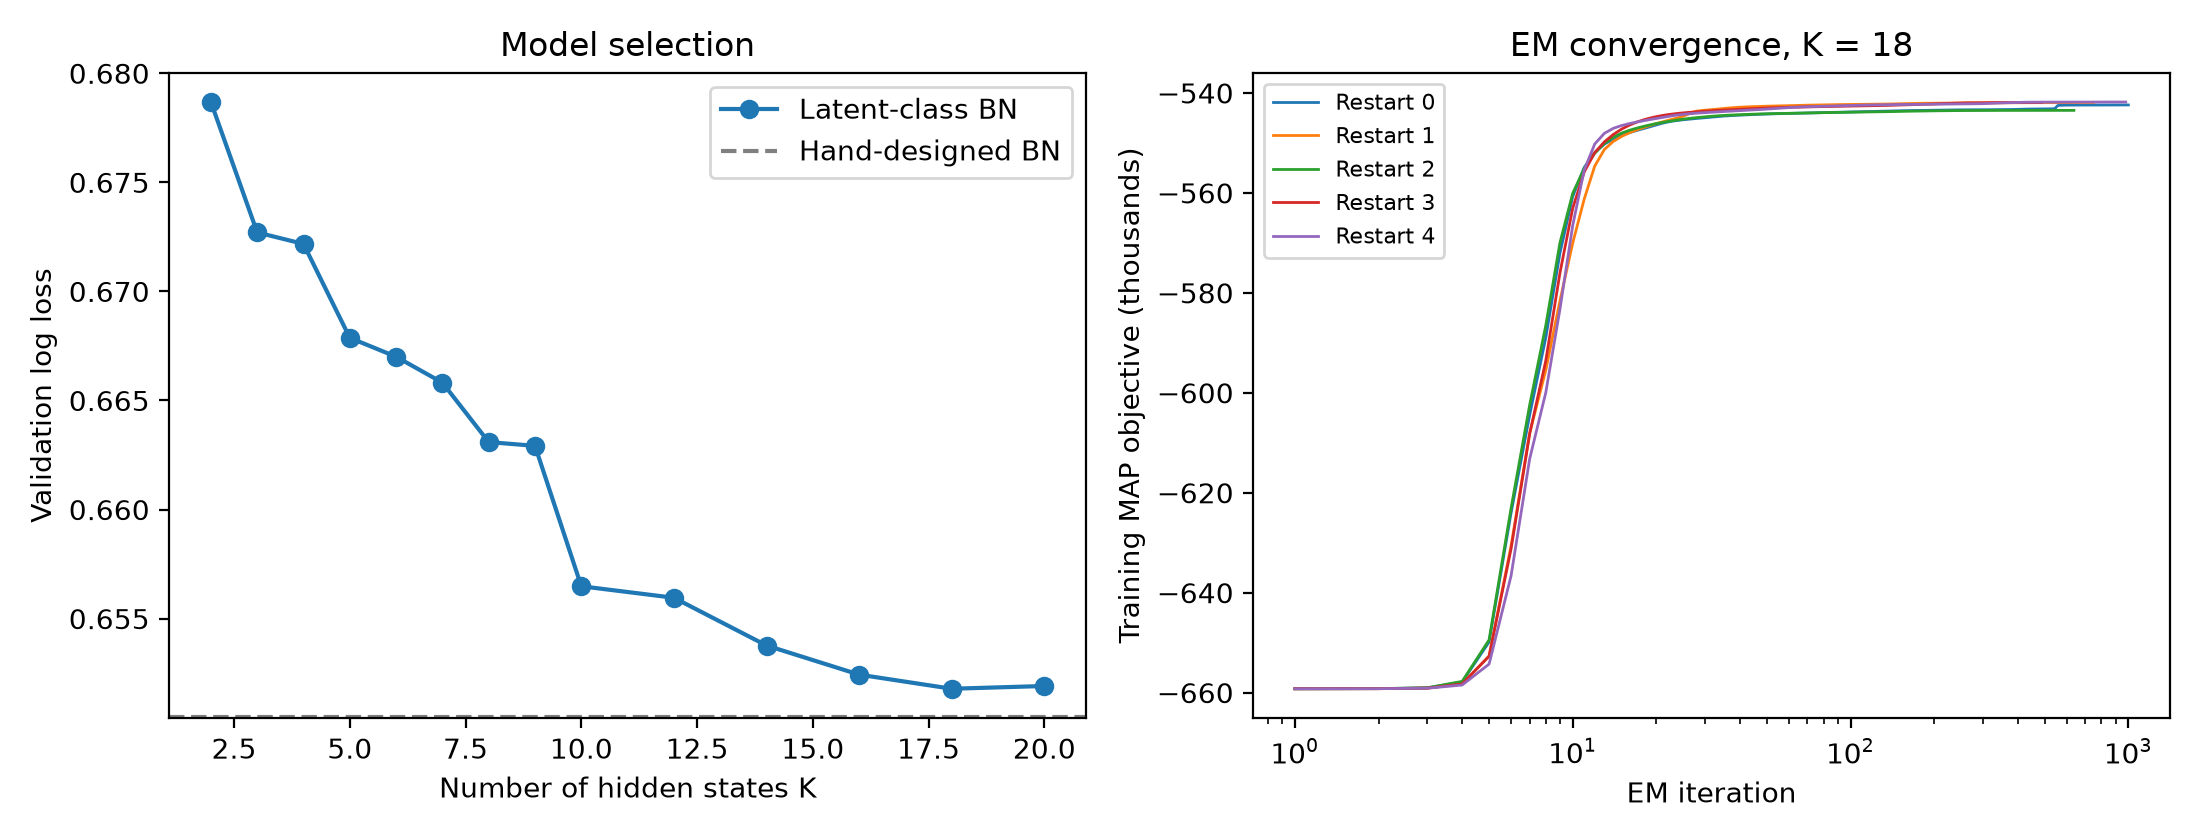
\includegraphics[width=\linewidth]{../results/figures/latent_em.png}
\caption{Validation selection and training-fit MAP-objective traces for the selected
$K$. Convergence is local and tolerance-based.}
\end{figure}

The leaves are independent only conditional on latent $Q$; marginalizing it can
represent observed feature dependence. Since $Q$ is unobserved, the earlier CMI
tests cannot directly test those conditional restrictions. State labels are
permutation-invariant and sorted by fitted make probability for display; modes
describe configurations, not identified causal difficulty or pure shooter ability.

\subsection{Player-level expected shooting}
For player $j$, $E_j=\sum_i p_{ij}$ and $\Delta_j=(A_j-E_j)/N_j$, where $A_j$
is actual makes. Every $p_{ij}$ is out-of-fold from the fixed hand CPT, using five
complete-game folds across all \CleanN{} cleaned shots/904 games. Stable shot
IDs, fold membership, and training-parent counts verify exclusion of each shot's
game; 13 full-analysis shots have unseen parent configurations. There are
\PlayerN{} players with at least 200 attempts. Player identity is used for
grouping, never for the prediction model.

For stability we split complete dates at \PlayerHalfDate{} and independently
cross-fit within each half. Thus one half's outcomes do not train the other's
residuals. The resulting $r=\PlayerHalfR{}$ is descriptive across \PlayerHalfN{}
players meeting the 100-attempt threshold in both halves, not a skill estimate
or an independent significance test. A saved Bernoulli-reference $z$ assumes
independent shots and known probabilities; clustering and model-estimation error
make it unsuitable as a calibrated significance claim.

\begin{table}[ht]
\caption{Illustrative players from the team's draft, reproduced using game-cross-fitted
probabilities. Gaps are actual minus expected field goal percentage, in percentage points.}
\centering\small\begin{tabular}{lrrrr}
\toprule
Player & Shots & Actual FG & Expected FG & Gap (pp)\\
\midrule
Stephen Curry & 965 & 48.6\% & 40.6\% & +8.0\\
Kyle Korver & 458 & 48.9\% & 37.6\% & +11.3\\
Klay Thompson & 967 & 46.3\% & 41.0\% & +5.3\\
\bottomrule
\end{tabular}

\end{table}
\begin{figure}[ht]
\centering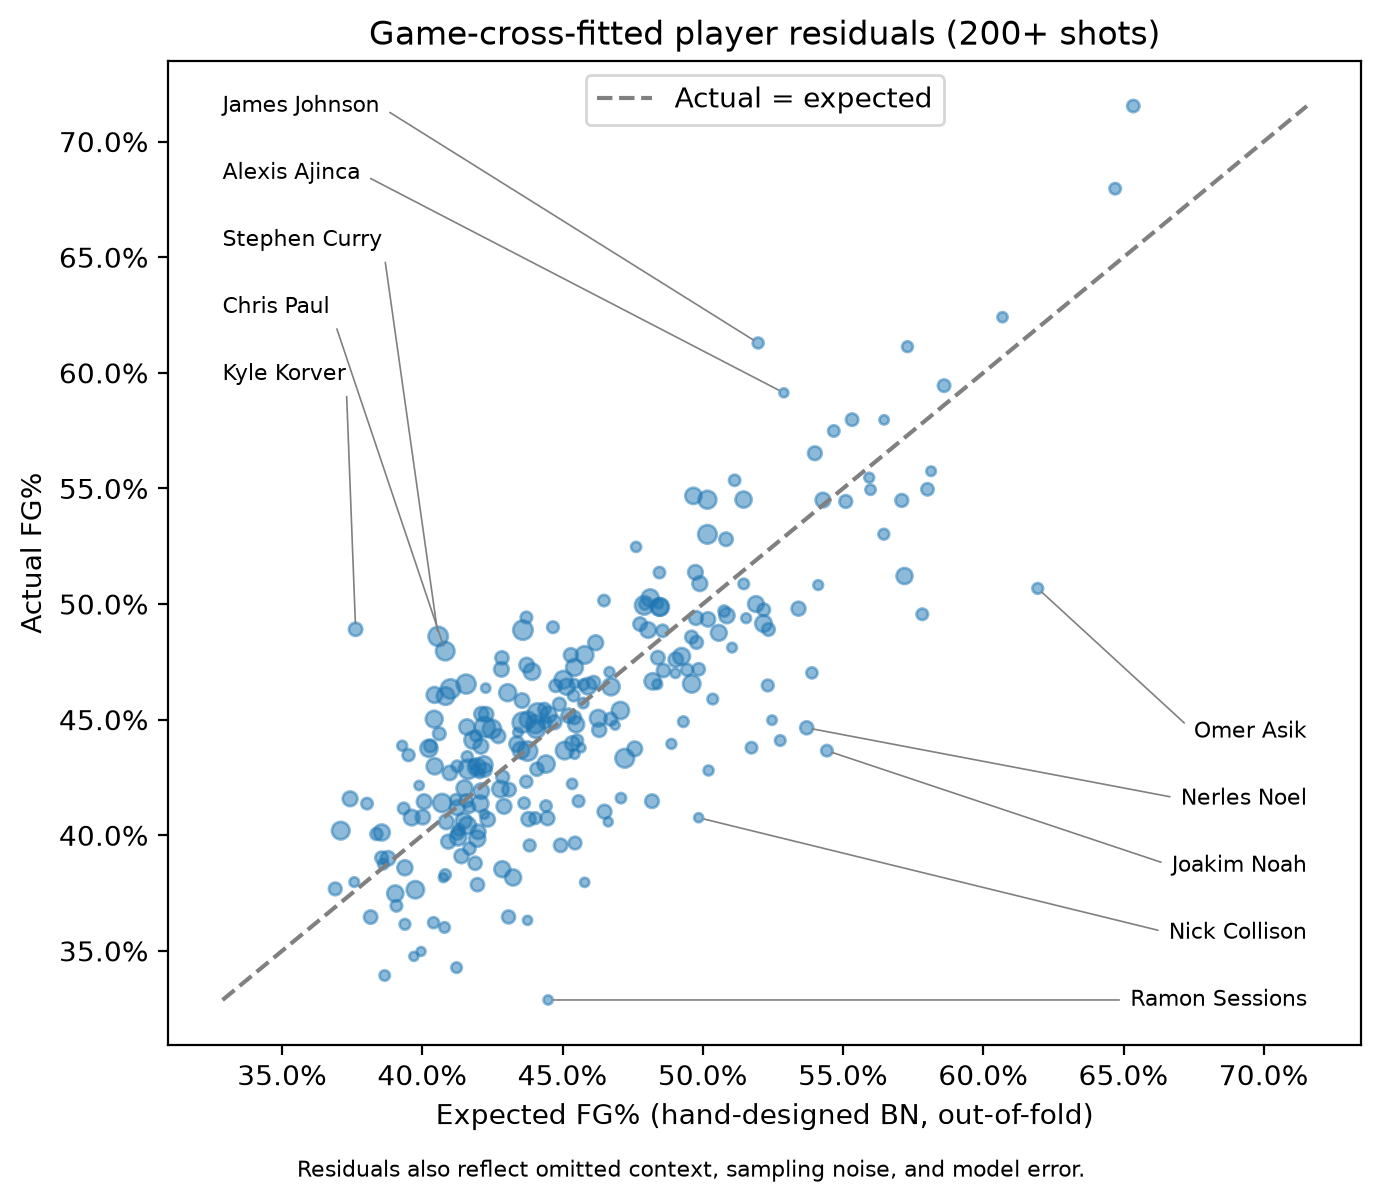
\includegraphics[width=0.85\linewidth]{../results/figures/player_actual_vs_expected.png}
\caption{Player residuals against the hand BN. Marker area reflects attempts;
extreme residuals can reflect omitted context and model error as well as shooting.}
\end{figure}

\subsection{Final team review before submission}
Complete individual statements/reflections, confirm any instructional feedback,
and review the code, findings, and AI disclosure in the team's own words.
Recompile after editing and keep Sections 1--6 within seven pages;
references and appendices are outside that limit. This draft has not been
submitted to Gradescope and no submission is implied by the PR.
\end{document}
